\documentclass[prl,12pt,onecolumn,nofootinbib,notitlepage,english,superscriptaddress]{revtex4-1}
\renewcommand{\rmdefault}{cmr}
\usepackage[T1]{fontenc}
\usepackage[latin9]{inputenc}
\setcounter{secnumdepth}{2}
\setcounter{tocdepth}{2}
\usepackage{color}
\usepackage{babel}
\usepackage{latexsym}
\usepackage{float}
\usepackage{amsmath}
\usepackage{amsfonts}
\usepackage{graphicx}
\usepackage{times}   %% Times Roman font
\usepackage{esint}
\usepackage{subfigure}
\usepackage{verbatim}
\usepackage{braket}
\usepackage{footmisc}
\usepackage[unicode=true,pdfusetitle,
 bookmarks=false,colorlinks=true,citecolor=blue,urlcolor=blue,linkcolor=red]{hyperref}
\makeatletter
%%%%%%%%%%%%%%%%%%%%%%%%%%%%%% LyX specific LaTeX commands.
\special{papersize=\the\paperwidth,\the\paperheight}

%%%%%%%%%%%%%%%%%%%%%%%%%%%%%% Textclass specific LaTeX commands.
\@ifundefined{textcolor}{}
{%
 \definecolor{BLACK}{gray}{0}
 \definecolor{WHITE}{gray}{1}
 \definecolor{RED}{rgb}{1,0,0}
 \definecolor{GREEN}{rgb}{0,1,0}
 \definecolor{BLUE}{rgb}{0,0,1}
 \definecolor{CYAN}{cmyk}{1,0,0,0}
 \definecolor{MAGENTA}{cmyk}{0,1,0,0}
 \definecolor{YELLOW}{cmyk}{0,0,1,0}
}

\@ifundefined{date}{}{\date{}}
\AtBeginDocument{
  \def\labelitemi{\(\rhd\)}
}
\makeatother

\setlength{\belowcaptionskip}{-7pt}
\newcommand{\SAVE}[1]{}
\newcommand{\HJC}[1]{{\color{RED}{\bf HJC: #1}}}
\newcommand{\prlsec}[1]{\emph{#1---}}
\newcommand{\Ncal}{{\mathcal N}}
\newcommand{\T}{{\mathbf{T}}}
\newcommand{\Jbq}{{J_{bq}}}
\newcommand{\DK}[1]{{\color{BLUE}{\bf DK: #1}}}

\begin{document}
\renewcommand{\thefootnote}{\fnsymbol{footnote}}
\renewcommand\abstractname{}
\title{From real materials to model lattice Hamiltonians: multi-scale modelling of strongly correlated electronic systems 
       with information from many body wavefunctions}

\author{Hitesh J. Changlani}
\affiliation{Department of Physics and Astronomy, Johns Hopkins University, Baltimore, Maryland 21218, USA}
\author{Huihuo Zheng}
\affiliation{
Argonne Leadership Computing Facility, Argonne National Laboratory, 9700 South Cass Avenue, Lemont, 60439, Illinois, USA}
\author{Kiel Williams}
\affiliation{Department of Physics and Institute for Condensed Matter Theory, University of Illinois at Urbana-Champaign, 
1110 West Green St, Urbana IL 61801, USA}
\author{Brian Busemeyer}
\affiliation{Department of Physics and Institute for Condensed Matter Theory, University of Illinois at Urbana-Champaign, 
1110 West Green St, Urbana IL 61801, USA}
\author{Lucas K. Wagner}
\affiliation{Department of Physics and Institute for Condensed Matter Theory, University of Illinois at Urbana-Champaign, 
1110 West Green St, Urbana IL 61801, USA}
\date{\today}
\maketitle

\textbf{
Given a realistic material with all its intrinsic complications, how does one develop a 
simple reliable model for understanding its properties? Theoretical insight has been the key driver of 
this process leading to simple few-band pictures. When the interactions are comparable 
to or much stronger than the kinetic energy, it is convenient to adopt the real space lattice 
approach and work with Hubbard or Kanamori type Hamiltonians involving only the low energy electrons. 
But this is no easy task, since the effective Hamiltonian involves a considerable renormalization of parameters with respect 
to the bare Coulomb values. While the kinetic energy is dominated by contributions from bands or states energetically 
near the Fermi level, screened interactions depend on states even \emph{far} away from it, leading to Hubbard U's 
that have been traditionally hard to reliably determine. 
Here we discuss an approach that treats the kinetic and potential parts of the Hamiltonian 
democratically and one that provides a transparent way of obtaining effective Hamiltonians using data from many body wavefunctions, 
and whose validity can be systematically checked.
We emphasize that determining the effective Hamiltonian reliably is crucial for 
several applications in physics and chemistry not only for quantitative accuracy, but also a 
correct qualitative picture of strongly correlated materials. 
}

\section{Introduction to downfolding the many electron problem}

In multiscale modeling of many-particle systems, the effective Hamiltonian (or Lagrangian) is one of the most core concepts. 
The effective Hamiltonian dictates the behavior of the system on a coarse-grained level, where `sub-grid' effects are folded into the parameters and form of the effective Hamiltonian. 
Many concepts in condensed matter physics can be viewed as statements about the behavior of the effective Hamiltonian. 
In particular, identification of `strongly correlated' materials as materials where band theory is not an accurate representation of the systems is a statement about effective Hamiltonians.
Effective Hamiltonians at different length scales also form the basis of the renormalization group~\cite{Wilson}.
A major goal in condensed matter physics is to determine what effective Hamiltonians apply to different physical situations, in particular quantum effective Hamiltonians, which lead to large-scale emergent quantum behavior. 

The dominant effective model for quantum particles in condensed systems is band structure, and for metals, Fermi liquid theory. 
However, a major challenge is how this paradigm should be altered when it is no longer a good description of the physical system.
Examples of these include the high-T$_c$ cuprates and other transition metal oxides, which do not appear to be well-described by these simple effective Hamiltonians. 
For these systems, many models have been proposed, such as the Hubbard~\cite{Hubbard1963}, Kanamori~\cite{Kanamori1963}, $t$-$J$~\cite{tJSpalek} and Heisenberg models.
While these models have been extensively studied analytically and numerically, and have significantly enhanced our understanding of the physics of correlated electrons, their effectiveness for describing a real complex system of interest is often unclear. 
At the same time, more complex effective models can be commensurately more difficult to solve,  so one would like to also find an accurate effective model that is tractable. 

%\begin{figure}
%\centering
%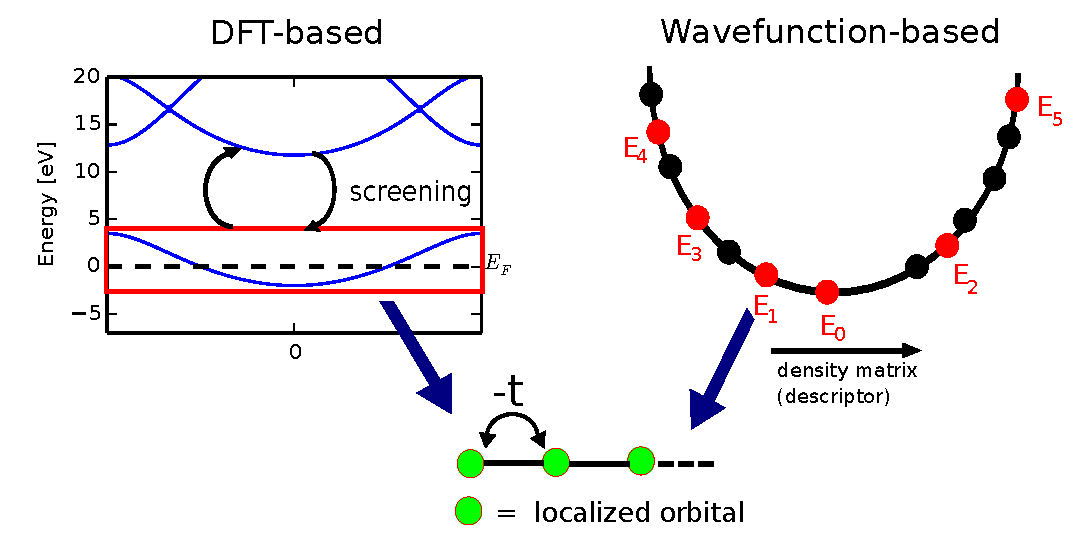
\includegraphics[width=1\linewidth]{./Figures/figure1.eps}
%\caption{Schematics for downfolding a simple ab-initio system (here the hydrogen chain) in DFT based methods (left) and the wave function based DMD (right). 
%Localized one particle functions are constructed in both methods and serve as the one body space for the model Hamiltonian. 
%The DFT based methods use Kohn Sham orbitals and screening models to estimate the interactions. 
%DMD uses a database of low energy all electron many-body wave functions ($\psi_i$). 
%This ``low energy basin" (shown abstractly in the space of descriptors) need not consist of exact eigenstates ($E_i$).\lucas{The energy should be a linear function of the density matrix!}}
%\label{fig:lowenergybasin_schematic}
%\end{figure}	

To address the need for a link between {\it ab-initio} electron-level models and larger scale models, downfolding has most commonly been carried out using approaches based on density functional theory (DFT). 
The kinetic part\BDB{kinetic part of what?} \HHZ{using single-body terms instead?}is obtained from a standard DFT calculation which is projected onto localized Wannier functions and gives an estimate of the effective hoppings of the lattice model based on Kohn-Sham band structure calculations~\cite{Pavirini}. 
Then, to estimate the interactions, one assumes a model of screening of the Coulomb interactions based on constrained DFT, RPA, or some other methods. 
Since effects of interactions between the orbitals of interest have already been accounted for by DFT, a double counting correction is required to obtain the final downfolded Hamiltonian. 
The approach has been developed and widely applied~\cite{Pavirini, Dasgupta, Aryasetiawan2004, Jeschke2013}; but remains an active area of research~\cite{Haule_doublecounting}.
There are other downfolding approaches that include the traditional L\"owdin method, coupled to a stochastic approach~\cite{Tenno,Zhou_Ceperley} and the related method of canonical transformations~\cite{White_CT, Yanai_CT}. 
While they have many advantages, it is typically not possible to know if a given model {\it ansatz} was a good guess or not, and it is very rare for a technique to provide an estimate of the quality of the resultant model. 

The situation described above stands in contrast to the derivation of effective classical models. 
For concreteness, let us discuss classical force fields computed from {\it ab initio} electronic structure calculations. 
Typically, a data set is generated using an {\it ab initio} calculation in which the positions of the atoms and molecules are varied, creating a set of positions and energies. 
The parameters in the force field {\it ansatz} are varied to obtain a best-fit classical model.
Then, using standard statistical tools, it is possible to assess how well the fit reproduces the {\it ab initio} data within the calculation, without appealing to experiment. 
While translating that error to error in properties is not a trivial task\lucas{citations}, this approach has the important advantage that in the limit of a high quality fit and high quality {\it ab initio} results, the resultant model is predictive.

Na\"ively, one might think to reconcile the fitting approach used in classical force fields with quantum models by matching eigenstates between a quantum model and {\it ab initio} systems, varying the model parameters until the eigenstates match~\cite{Wagner2013}. 
However, this strategy does not work well in practice because it is often not possible to obtain exact eigenstates for either the model or the {\it ab initio} system.
To resolve this, we develop a general theory for generating effective quantum models that is exact when the wave functions are sampled from the manifold of low-energy states. 
Because this method is based on fitting the energy functional, 
We will show the practical application of this theory using both exact solutions and {\it ab-initio} quantum Monte Carlo (QMC) to derive several different quantum models.


The endeavor we pursue here is to develop a multi-scale approach in which the effective interactions between quasiparticles (such as dressed electrons) are determined after an \textit{ab-initio} simulation (but not necessarily exact solution) of the continuum Schroedinger equation involving all the electrons. 
The method uses reduced density matrices (RDMs) of low-energy states, not necessarily eigenstates, 
to cast downfolding as a fitting problem. 
We thus call it density matrix downfolding (DMD).
In this paper, these states will typically be generated using QMC techniques [either variational Monte Carlo (VMC) or diffusion Monte Carlo (DMC)] to come close to the low energy manifold.
The remainder of the paper is organized as follows:
\begin{itemize} 
\item 	In Section 2, we clarify and make precise what it means to downfold 
a many-electron problem to a few-electron problem. We recast the problem into minimization 
of a cost function that needs to be optimized to connect the many and few body problems. We further 
these notions both in terms of physical as well as information science descriptions, which allows us to connect to compression algorithms in the machine learning literature. 
\item Section 3 discusses several representative examples where we consider multiband lattice models 
and ab-initio systems to downfold to a simpler lattice model. 
\item In Section 4, we discuss future prospects of applications of the DMD method, ongoing challenges 
and clear avenues for methodological improvements. 
\end{itemize}



%\newtheorem{theorem}{Theorem}
\newtheorem{definition}{Definition}


\section{Downfolding as a compression of the energy functional}
\label{sec:theory}
\subsection{Theory} 

Suppose we start with a quantum system with Hamiltonian $H$ and Hilbert space ${\mathcal H}$.

\begin{definition}
Let the energy functional be $E[\Psi] = \frac{\bra{\Psi}H\ket{\Psi}}{\braket{\Psi|\Psi}}$ for a wavefunction $\ket{\Psi} \in {\mathcal H}$.
\end{definition}


\begin{definition}
Let ${\mathcal LE}(H,N)$ be a subset of ${\mathcal H}$ spanned by $N$ vectors given by the lowest energy solutions to $H\ket{\Phi_i}=E_i{\Phi_i}$. 
\end{definition}

\begin{definition}
$H_{eff}$ is an operator on the Hilbert space ${\mathcal LE(H,N)}$.	 
\end{definition}


\begin{definition}
The effective model $E_{eff}[\Psi]=\frac{\bra{\Psi}H_{eff}\ket{\Psi}}{\braket{\Psi|\Psi}}$ is a functional from ${\mathcal LE} \rightarrow \mathbb{R}$
\end{definition}



\begin{theorem}
\label{theorem:criticalpoint}
$E[\Psi]$ has a critical point only where $\Psi$ is an eigenstate of $H$.
\end{theorem}
\begin{proof}
\begin{eqnarray}
\frac{\delta }{\delta \Psi^*}  E[\Psi] = \frac{\delta}{\delta \Psi^*}\frac{\langle \Psi |H|\Psi\rangle}{\langle \Psi |\Psi\rangle} = \frac{H|\Psi\rangle}{\langle \Psi |\Psi\rangle} - \langle \Psi |H|\Psi\rangle \frac{|\Psi \rangle}{|\langle \Psi | \Psi\rangle|^2} =\frac{ (H-E[\Psi])|\Psi\rangle }{\langle\Psi|\Psi\rangle}\,.
\end{eqnarray}
Therefore, 
$\frac{\delta }{\delta \Psi^*}  E[\Psi] = 0$ if and only if $(H-E[\Psi])|\Psi\rangle =0$, i.e., $\Psi$ is an eigenvector of $H$ corresponding to eigenvalue $E[\Psi]$.  
\end{proof}


%\begin{theorem} 	
%If $E_{eff}[\Psi] = E[\Psi], \forall \ket{\Psi} \in {\mathcal LE}$, then $H_{eff} \ket{\Phi_i} = E_i\ket{\Phi_i}$ for all eigenstates $\ket{\Phi_i}\in {\mathcal LE}$.
%\end{theorem}
%\begin{proof}
%	Suppose that $\ket{\Phi_i}$ is an eigenstate of $H$. Then 
%	\begin{equation}
%	\left.\frac{\delta E[\Psi]}{\delta\Psi}\right|_{\Psi=\Phi_i} = 0 
%	\end{equation}
%If this is true, then certainly the derivative on the low-energy manifold is also zero.
%\HJC{I am slightly confused. This is because the earlier derivative was in the space of all many body wavefunctions. But now the derivative is 
%constrained somehow because of loss of degrees of freedom.. }
%Since $E_{eff}[\Psi] = E[\Psi]$, 
%\begin{equation}
%	\left.\frac{\delta E_{eff}[\Psi]}{\delta\Psi}\right|_{\Psi=\Phi_i} = 0 
%\end{equation}
%for $\ket{\Psi} \in {\mathcal LE}$. Using Theorem~\ref{theorem:criticalpoint}, $H_{eff} \ket{\Phi_i} = E_i\ket{\Phi_i}$. 
%Similarly, if the derivative is not zero, then the wave function must not be an eigenstate.
%\end{proof}
\begin{theorem}
\label{theorem:matching}
Assume $\ket{\Psi } \in {\mathcal LE}$ and $E_{eff}[\Psi] = E[\Psi]$.
Then $H_{eff}\ket{\Psi}  = E \ket{\Psi} \iff H\ket{\Psi} = E\ket{\Psi}$.
\end{theorem}
\begin{proof}
Since $E_{eff}[\Psi] = E[\Psi]$, $\frac{\delta  E[\Psi] }{\delta \Psi^*}  = \frac{\delta E_{eff}[\Psi]}{\delta \Psi^*}  $.
If $\frac{\delta  E[\Psi] }{\delta \Psi^*} =0$, then $\frac{\delta E_{eff}[\Psi]}{\delta \Psi^*} =0$ since ${\mathcal LE}$ is a subset of ${\mathcal H}$.
If $\frac{\delta E_{eff}[\Psi]}{\delta \Psi^*} =0$, then write a state $\ket{\Phi}\in {\mathcal H} = \ket{\Psi} + \ket{\Psi_{HE}}$, where $\ket{\Psi}$ is the projection of $\ket{\Phi}$ into ${\mathcal LE}$. 
Then
\begin{align}
\left.\frac{\delta  E[\Phi] }{\delta \Phi^*}\right|_{\Phi=\Psi} =  \left[\frac{\delta  E[\Phi] }{\delta \Psi^*} + \frac{\delta  E[\Phi] }{\delta \Psi_{HE}^*} \right]_{\Phi=\Psi}.
\end{align}
\HHZ{This proof is not rigorous. if $y=a+b$, we don't have $\frac{\partial f}{\partial y} =\frac{\partial f}{\partial a} +\frac{\partial f}{\partial b} $. One needs to have rigorous chain rule to deduce some results like this. For example, define another variable $x=a-b$, ... }
$\frac{\delta  E[\Phi] }{\delta \Psi^*}=0$ because $\frac{\delta E_{eff}[\Psi]}{\delta \Psi^*} =0$. 
$\frac{\delta  E[\Phi] }{\delta \Psi_{HE}^*}=0$ can easily be verified by noting that $\ket{\Psi_{HE}}= \sum_{i=N+1}^\infty c_i \ket{\Phi_i}$.
Since the zeros coincide, the eigenstates also coincide. 
\end{proof}
\HHZ{The whole theorem does not work. You can see clearly if I write H as the following form, 
\begin{eqnarray}
H = 
\begin{pmatrix}
 H_{LE}  & H_c\\
H_c^\dagger & H_{HE}
\end{pmatrix}\,,
\end{eqnarray}
Then, based on all your definition, we have $H_{eff}=H_{LE}$. For sure this, satisfies the condition $E_{eff}[\Psi]= E[\Psi]$. But $H$ and $H_{eff}$ might not have coincide eigen spectrums if $H_c\ne0$. In other words, if and only if the high energy manifold and low energy manifold are decoupled with each other, we have coincide eigen spectrums for H and $H_{eff}$. 

In short, Theorem 2 does not work because when we apply $H$ to $\Psi$ (belong to LE), it in general will generate HE components. This is the same concern that Hitesh expressed in his comment. 
}

We have thus reduced the problem of finding an effective Hamiltonian $H_{eff}$ that reproduces the low-energy spectrum of $H$ to matching the corresponding energy functionals $E[\Psi]$ and $E_{eff}[\Psi]$. 
This involves both choosing the form of $H_{eff}$ and optimizing the parameters.
An important implication of this is that it is not necessary to diagonalize either of the Hamiltonians; one must only be able to select wave functions from the low-energy space ${\mathcal LE}$.
As we shall see, this can be substantially easier than attaining eigenstates.


The theory presented above maps coarse-graining into a functional approximation problem. 
This is still rather intimidating, since even supposing one can generate wave functions in the low-energy space, they are still complicated objects in a very large space.
An effective way to accomplish this is through the use of descriptors, $d_i[\Psi]$, which map from ${\mathcal H} \rightarrow \mathbb{R}$.
Then we can approximate the energy functional as follows
\begin{equation}
E_{eff}[\Psi] \simeq \sum_i f_i(d_i[\Psi]),
\end{equation}
where $f_i$ are some parameterized functions.
This will allow us to use techniques from statistical learning to efficiently describe $E_{eff}$. 
\subsection{Practical protocol}

\tikzstyle{decision} = [diamond, draw, fill=blue!10, 
    text width=4.5em, text badly centered, node distance=3cm, inner sep=0pt]
\tikzstyle{block} = [rectangle, draw, fill=blue!10, 
    text width=5em, text centered, rounded corners, minimum height=4em]
\tikzstyle{result} = [rectangle, draw, fill=red!10, 
    text width=5em, text centered, rounded corners, minimum height=4em]
\tikzstyle{line} = [draw,-latex',very thick]
\tikzstyle{cloud} = [draw, ellipse,fill=red!20, node distance=3cm,
    minimum height=2em]
\begin{figure*}
\begin{tikzpicture}[scale=2,node distance = 3cm, auto]
    % Place nodes
    \node [block] (wfs) {Generate $\ket{\Psi_i} \in {\mathcal LE}$};
    \node [block, right of=wfs] (descriptors) {Generate $d_j[\Psi_i]$,$E[\Psi_i]$};
    \node [block, right of=descriptors] (assess) {Assess descriptors};
    \node [block, right of=assess] (ansatz) {Ansatz: $E_i \simeq \sum_j p_j d_{ij}$};
    \node [block, right of=ansatz] (fit) {Fit optimal model};
    \node [result, right of=fit] (model) {Effective model};
    % Draw edges
    \path [line] (wfs) -- (descriptors);
    \path [line] (descriptors) -- (assess);
    \path [line] (assess) --  (ansatz);
    \path [line] (ansatz) --  (fit);
    \path [line] (fit) --  (model);

    \path [line] (assess.south) -- ($ (assess.south) + (0,-0.2)$) 
                 -- node [below] {Incomplete sampling} 
                 ($ (wfs.south) + (0,-0.2)$) --  (wfs.south);
    \path [line] (assess.north) -- ($ (assess.north) + (0,0.2)$) 
                 -- node [above] {Incomplete descriptor space} 
                 ($ (descriptors.north) + (0,0.2)$) --  (descriptors.north);

\end{tikzpicture}
\caption{A practical protocol for fitting effective models to {\it ab initio} data.}
\label{fig:protocol} 
\end{figure*}

A practical protocol is presented in Fig~\ref{fig:protocol}. 
In this section we go through this procedure step by step.

\paragraph{Generating $\ket{\Psi_i}\in {\mathcal LE}$}
Ideally one would be able to sample the entire low-energy space. 
Typically, however, the space will be too large and it will need to be sampled. 
The optimal wave functions to use depend on the models one expects to fit, which we will discuss in detail  in later steps. 
Simple strategies that we will use in the examples below include excitations with respect to a determinant and varying spin states.


\paragraph{Generate $d_j[\Psi_i]$ and $E[\Psi_i]$} 
The choice of descriptor is fundamental to the success of the downfolding. 
In the case of a second-quantized Hamiltonian
\begin{equation}
\hat{H}_{eff} = E_0 + \sum_{ij} t_{ij} (c_i^\dagger c_j + h.c.) + \sum_{ijkl} V_{ijkl} c_i^\dagger c_j^\dagger c_k c_l,
\end{equation}
a set of linear descriptors by simply taking the expectation value of both sides of the equation. 
Then for example, the occupation descriptor for orbital $k$ is $d_{occ(k)}[\Psi_i] = \braket{\Psi_i | c_k^\dagger c_k | \Psi}$; the double occupation descriptor for orbital $k$ is $d_{double(k)}[\Psi_i] = \braket{\Psi_i | n_{k\uparrow}n_{k\downarrow} | \Psi}$. 
The orbital that $c_k$ represents is part of the descriptor, and in the examples below we will discuss this choice as well.
One is not limited to static orbital descriptors; they may have a more complex functional dependence on the trial function to include orbital relaxation.

 
\paragraph{Assess descriptors}
At this point, one has collected the data $E_i$ and $d_{ij}$. 
If two descriptors have a large correlation coefficient, then they are redundant in the data set. 
This could either mean that the sampling of the low-energy Hilbert space ${\mathcal LE}$ was insufficient, or that they are both proxies for the same differences in states. 
If two data points have the same or very similar descriptor sets, but different energies, then either the descriptor set is not enough to describe the variations in the low-energy space, or the sampling has generated states that are not in the low-energy space.
To resolve these possibilities, one should analyze the difference between the two wave functions.  
Choosing the reduced set requires some intuition or somewhat advanced analysis of the many possibilities. 
In either case, when the model is accurate, the fits will be accurate.
If they are chosen incorrectly then intruder states can appear upon solution of the effective model. 
This can occur if descriptors values available in the reduced Hilbert space are not represented in the sampled wave functions. 
In that case, the model fitting is an extrapolation instead of an interpolation, which has the usual problems.
This is why it is desirable to have eigenstates in the set if possible; they are guaranteed to be on the corners of the descriptor space if the model is accurate.


\paragraph{Ansatz: $E_i \simeq \sum_i  d_{ij} p_j$} 
If the descriptors are chosen well, then the model can be written in linear form:
\begin{equation}
E[\Psi_i] = \sum_j p_j d_j[\Psi_i],	
\end{equation}
which we shorten to 
\begin{equation}
{\bf E} = D{\bf p} .
\label{eqn:EdP}
\end{equation}
If this can be done, the fitting problem is reduced to a linear regression optimization.
More complex functions of the descriptors are also possible, although at the cost of making the effective model more difficult to solve and complicating the fitting procedure.


\paragraph{Fit optimal model}
Finally, one wishes to find a set of parameters such that Eqn~\ref{eqn:EdP} is satisfied as closely as possible. 
There are many choices to make in this step, which will often depend on the desired properties of the final model. 
One can imagine choosing different cost functions to minimize, which can also include a penalty for complicated models. 
In our tests, we have successfully used LASSO \cite{Lasso} and matching pursuit techniques \cite{MP_Zhang1993} to select high quality and compact model parameters. 
A detailed example of using the latter technique is presented in Section~\ref{subsection:fese}.



\section{Theory: Compression of the Energy Functional/Criteria for Hamiltonian matching}
\HJC{Lucas handling this section......Look at theory.tex. Could use commented out snippets explaining Ax=E etc and criteria}
\section{Representative Examples}

Given the theoretical framework for downfolding a many-orbital (or many electron) problem to a 
few orbital (or few electron) problem, we now discuss few examples which also serve to highlight some practical aspects 
associated with AIDMD. The first example is mostly pedagogical, 
where we have completely avoided the \textit{ab-initio} related complications of AIDMD. Rather, we use information directly available 
from \textit{exact} eigenstates themselves to downfold from a lattice model with more orbitals (3-band model) 
to one with fewer orbitals (1-band model). We then gradually increase the complexity of the problems we address 
by downfolding the hydrogen chain in one dimension (with up to 10 atoms) and graphene 
(with up to 32 carbons on a 2D honeycomb lattice). \lucas{don't forget FeSe}

\lucas{This paragraph seems somehow out of place to me. While it is true that the choice of the orbitals is important, so is the choice of the effective Hamiltonian and the sampling of the low energy space. This is a good place to point out that one should be looking for those things. }A common occurrence\lucas{For 3/4 of our examples..} in most of our examples is the 1-band Hubbard Hamiltonian, defined as,
\begin{equation}
	\tilde{H} = -t \;\sum_{\langle i,j \rangle} \tilde{d}_i^{\dagger} \tilde{d}_j + U \;\sum_{i} \tilde{n}^{i}_{\uparrow} \tilde{n}^{i}_{\downarrow}
\label{eq:oneband}
\end{equation}
where $t$ and $U$ correspond to downfolded (renormalized) parameters and $\tilde{d}$ are the effective one-particle operators, 
which are obtained from transformations on their bare counterparts. 
This choice is crucial for obtaining accurate Hamiltonians and we highlight it for each example presented.   

\subsection{Three-band Hubbard model to one band Hubbard model at half filling}

Our first example is motivated by the high $T_c$ superconducting cuprates~\cite{Bednorz1986} that 
have parent Mott insulators with rich phase diagrams on electron or hole doping~\cite{Dagotto_RevModPhys, LeeWen_RevModPhys}. 
Many works have been devoted to their model Hamiltonians and corresponding parameter 
values~\cite{Emery, ZhangRice, tJSpalek, Hybertsen_PRB1989, Hybertsen_PRB1990, Pavirini, Kent_Hubbard}. 
The emergent consensus of the minimal model involving the oxygens is the 3-orbital or 3-band Hubbard model, 
\begin{eqnarray}
H &=&    \epsilon_p \sum_{j,\sigma} n^{p}_{j,\sigma} + \epsilon_{d} \sum_{i,\sigma}  n^{d}_{i,\sigma} 
	+ t_{pd} \sum_{\langle i,j \rangle, \sigma} \text{sgn}(p_i,d_j) \Big( d_{i,\sigma}^{\dagger} p_{j,\sigma} + \text{h.c.} \Big) \nonumber \\
  & &   + U_p \sum_{j} n^{p}_{j,\uparrow} n^{p}_{j,\downarrow} + U_d \sum_{i} n^{d}_{i,\uparrow} n^{d}_{i,\downarrow} + V_{pd} \sum_{\langle i,j \rangle} n^{j}_p n^{i}_d 
\end{eqnarray}
where $d_i,p_j$ refer to the  $d_{x^2 - y^2}$ orbitals of copper (at site $i$) and $p_x$ or $p_y$ 
oxygen (at site $j$)  respectively and the signs of the hopping $t_{pd}$ between them are shown in Fig.~\ref{fig:threeband}. 
$\epsilon_d$,$\epsilon_p$ refer to the orbital energies, 
$U_d$, $U_p$ refer to strength of onsite Hubbard interactions and $V_{pd}$ refers to the 
strength of the density-density interactions between a neighboring $p$ and $d$ orbital. 
We keep the exposition simple and consider only the case where $\epsilon_p$, $t_{pd}$ and $U_{d}$ are non zero
(since we work with fixed number of particles we set $\epsilon_d = 0$). 
The charge transfer energy $\Delta \equiv \epsilon_p - \epsilon_d$ equals $\epsilon_p$ in our notation. 
We work in the hole notation; half filling corresponds to 2$\uparrow$ and 2$\downarrow$ 
holes on the $2\times2$ cell.

\begin{figure}[htpb]
\centering
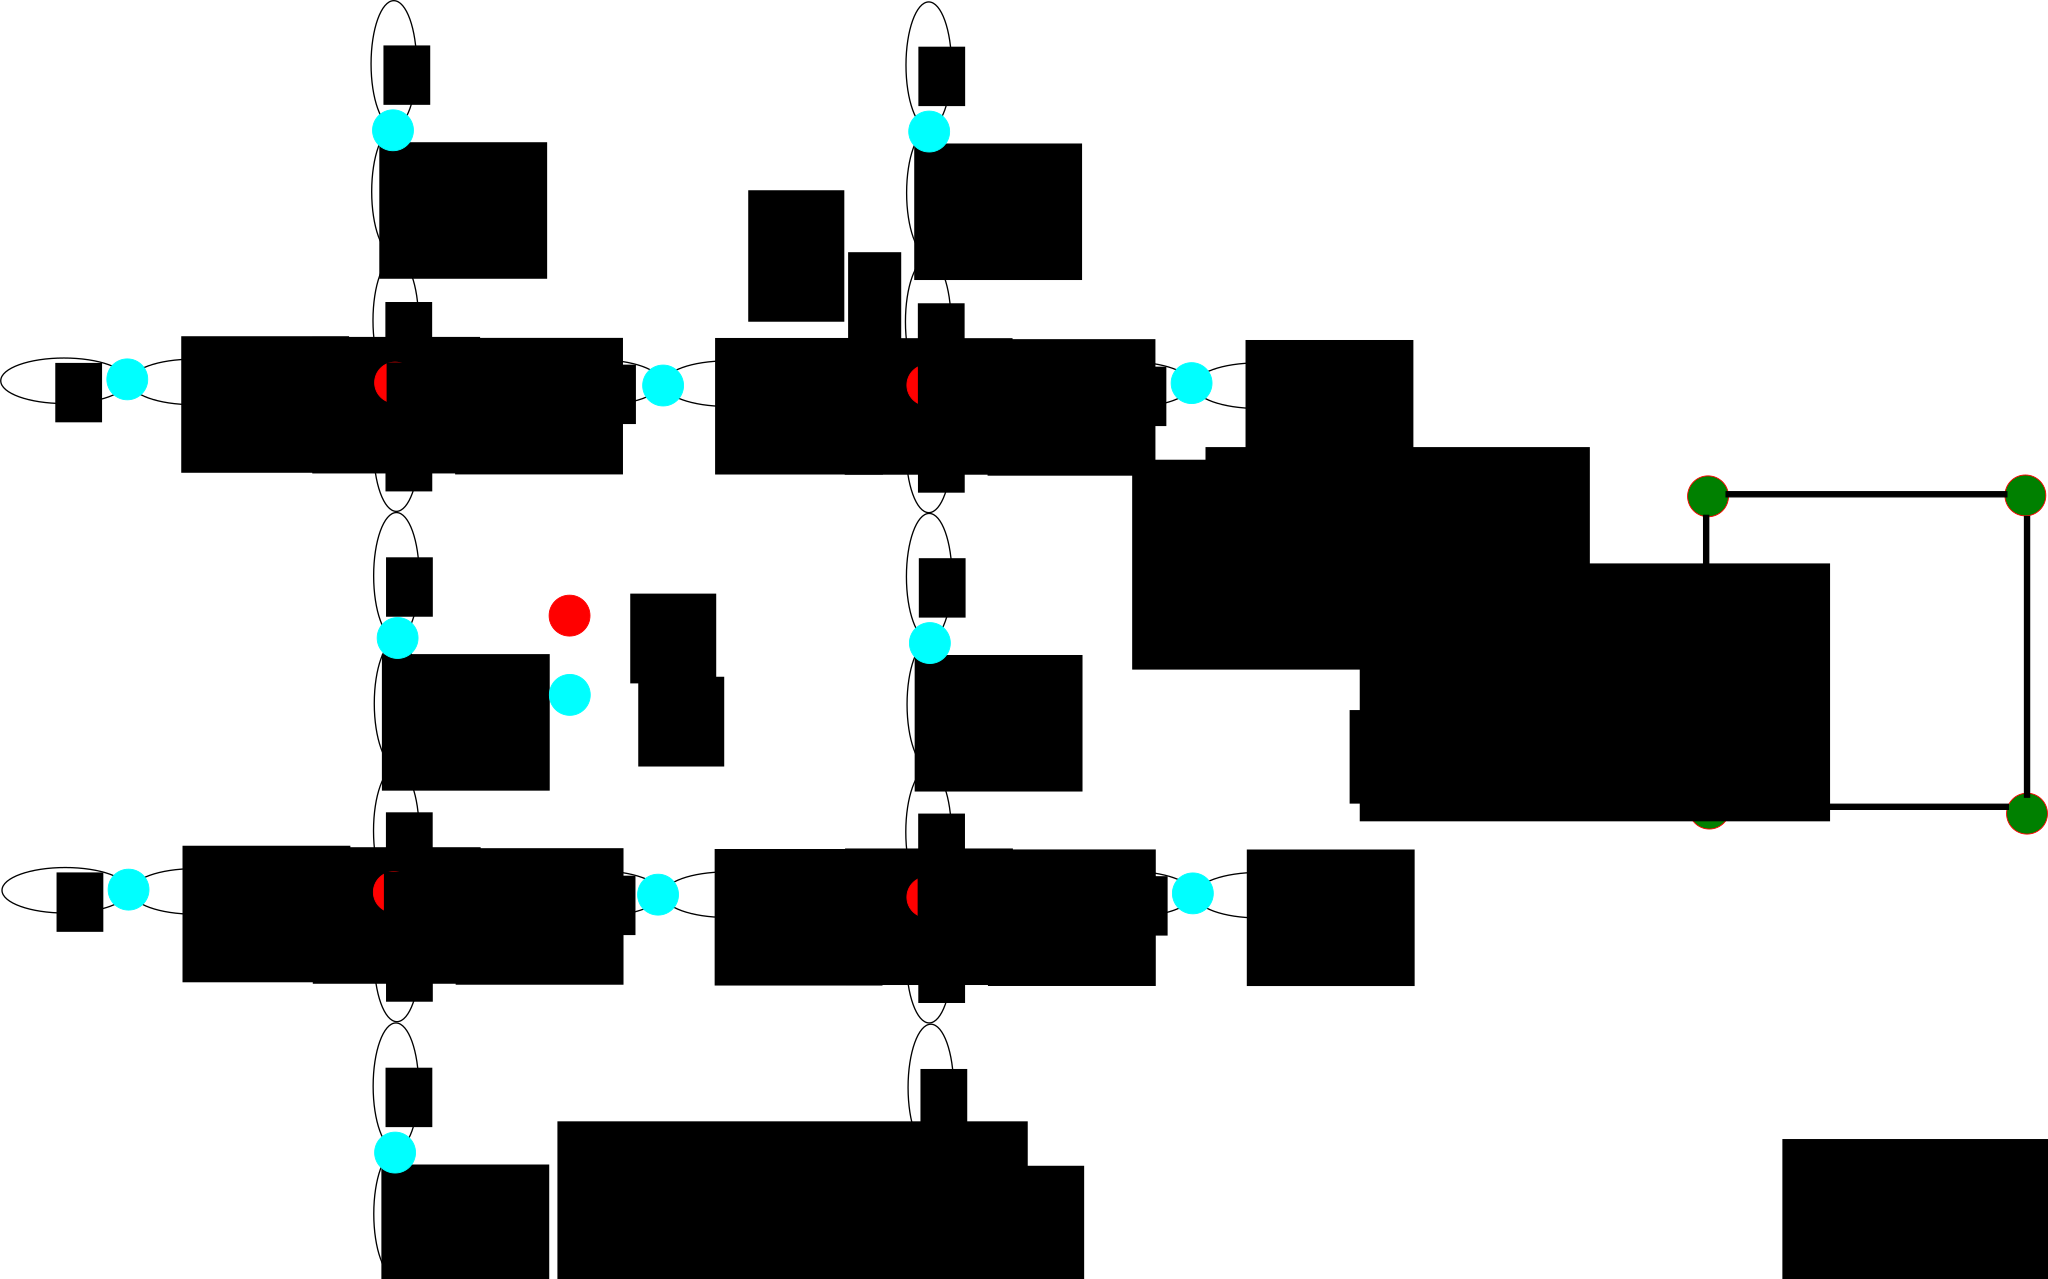
\includegraphics[width=0.8\linewidth]{./Figures/three_band_figure.pdf}
\caption{Schematic for downfolding the three band Hubbard model to the one band Hubbard model. 
The oxygen orbitals are completely eliminated to give "dressed" $d$-like orbitals of the one band model, with modified hopping 
and interaction parameters.}
\label{fig:threeband} 
\end{figure}	

Here we determine what 1-band parameters best describe the 3-band data, the former defined 
in terms of effective \textit{d-like} orbitals, $\tilde{d}$, which are mixtures of copper and oxygen orbitals and this optimal transformation also remains an unknown. (This highlights that the determination of effective Hamiltonians is a \emph{dual} problem - 
what are the composite objects that give a compact description of the low energy physics? and given this choice what 
are the effective interactions between them?) Here we encode the relationship between the 
bare and effective operators as a linear transformation ${\bf T}$, 
\begin{equation}
	\tilde{d}_i = \sum_{j} T_{ij} c_j
\end{equation}
%where $\tilde{d}_i$ is a transformed hole (destruction) operator 
where $c_j$ is the bare hole (destruction) operator and refers to either the bare $d$ or $p$ orbitals. 
(Note that higher body generalizations are also possible, but have not been considered here). 
Accounting for all symmetries of the $2\times2$ unit cell, {\bf T} is a $4 \times 12 $ matrix (the numbering of the orbitals 
corresponds to Fig.~\ref{fig:threeband}) is explicitly written out as, 
\begin{eqnarray}
{\bf T} = 
\left(
\begin{array}{cccccccccccc}
F        & \alpha_2 &        \alpha_2 &  \alpha_4 & \alpha_1 & \alpha_1 & -\alpha_1 & -\alpha_1 & \alpha_3 & -\alpha_3 & \alpha_3 & -\alpha_3 \\
\alpha_2 &  F       &        \alpha_4 &  \alpha_2 & \alpha_3 & -\alpha_1 & \alpha_1 & -\alpha_3 & -\alpha_3 & \alpha_3 & \alpha_1 & -\alpha_1 \\
\alpha_2 & \alpha_4 & F               &  \alpha_2 & -\alpha_1 & \alpha_3 & -\alpha_3 & \alpha_1 & \alpha_1 & -\alpha_1 & -\alpha_3 & \alpha_3 \\
\alpha_4 & \alpha_2 & \alpha_2        &   F       & -\alpha_3 & -\alpha_3 & \alpha_3 & \alpha_3 & -\alpha_1 & \alpha_1 & -\alpha_1 & \alpha_1 \\
\end{array}
\right)
\end{eqnarray}
where we have defined $F \equiv \sqrt{1-4{\alpha_1}^2 - 2{\alpha_2}^2 - 4 {\alpha_3}^2 -{\alpha_4}^2}$ and 
where the parameters $\alpha_1$,$\alpha_2$,$\alpha_3$ and $\alpha_4$ will be optimized to minimize a 
certain cost function, which will be explained shortly. 

The one particle density matrix (calculated in eigenstate $s$) 
in the transformed basis is related to that in the original basis,
\begin{equation}
	\langle {\tilde{d}_i}^{\dagger} \tilde{d}_{j} \rangle_{s} = \sum_{mn} T^{*}_{im} \langle {c_m}^{\dagger} c_n \rangle_{s} T_{jn}
\end{equation}
Using this relationship, we demand two conditions be satisfied, (1) the effective orbitals ($\tilde{d}_i$) are orthogonal to each other 
and (2) all diagonal entries of the 1-RDM of the effective orbitals for all low energy eigenstates $(\langle {\tilde{d}_i}^{\dagger} \tilde{d}_{i} \rangle)$ equal 1/2. These conditions are enforced by minimizing a cost function,
\begin{equation}
	C = \sum_{s} \sum_{i} \Big( \langle {\tilde{d}_i}^{\dagger} \tilde{d}_{i} \rangle_{s} - \frac{1}{2} \Big)^{2} + \sum_{mn} ( \Big({\bf T} {\bf T}^{\dagger}\Big)_{mn} -\delta_{mn})^{2}
\end{equation} 

To give a concrete and representative example of our results, we optimize the transformation 
according to Eq. and find the optimal parameters $\alpha_1=0.220$, $\alpha_2=0.044$, $\alpha_3=0.020$ 
and $\alpha_4=0.018$ 
\begin{small}
\begin{eqnarray}
\left(
\begin{array}{cccc}
+0.499 & -0.158 & -0.158 & 0.000  \\
-0.158 & +0.499 &  0.000 & -0.158 \\
-0.158 &  0.000 & +0.499 & -0.158 \\
 0.000 & -0.158 & -0.158 & +0.499 \\
\end{array}
\right);
\left(
\begin{array}{cccc}
+0.498 & -0.141 & -0.141 & -0.001  \\
-0.141 & +0.498 & -0.001 & -0.141 \\
-0.141 & -0.001 & +0.498 & -0.141 \\
-0.001 & -0.141 & -0.141 & +0.498 \\
\end{array}
\right)
;\left(
\begin{array}{cccc}
+0.498 & -0.083 & -0.083 & -0.032  \\
-0.083 & +0.498 & -0.032 & -0.083 \\
-0.083 & -0.032 & +0.498 & -0.083 \\
-0.032 & -0.083 & -0.083 & +0.498 \\
\end{array}
\right)
\end{eqnarray}
\end{small}
We then ask $U/t$ of the 1-band Hubbard model best describes this transformed 
1-RDMs. This is state specific and we find $(U/t)_1 = $ 
The density matrix matching does not provide an absolute energy scale for the matching. 
Taking $t_{pd} = 1.3$ eV, we then optimize $t$ (with fixed $(U/t)_2$ obtained from the procedure described 
previously) to best fit the energy spectra between the two models. This gives the optimal value of 
$t$. 


\begin{figure}[]
\centering
\includegraphics[width=0.49\linewidth]{./Figures/Hyb_vs_ep_Ud_8.pdf}
\includegraphics[width=0.49\linewidth]{./Figures/U_and_hopping_combined_vs_ep_Ud_8.pdf}
\caption{(Left) Optimized values of parameters entering the transformation matrix 
($\alpha_1$ through $\alpha_4$) and (Right) Effective 1-band Hubbard $U/t$ and hopping $t$ (inset) 
versus $\Delta/t_{pd}$ for fixed $U_{d}/t_{pd}=8$}
\label{fig:hamfitepdvary} 
\end{figure}	

\begin{figure}[]
\centering
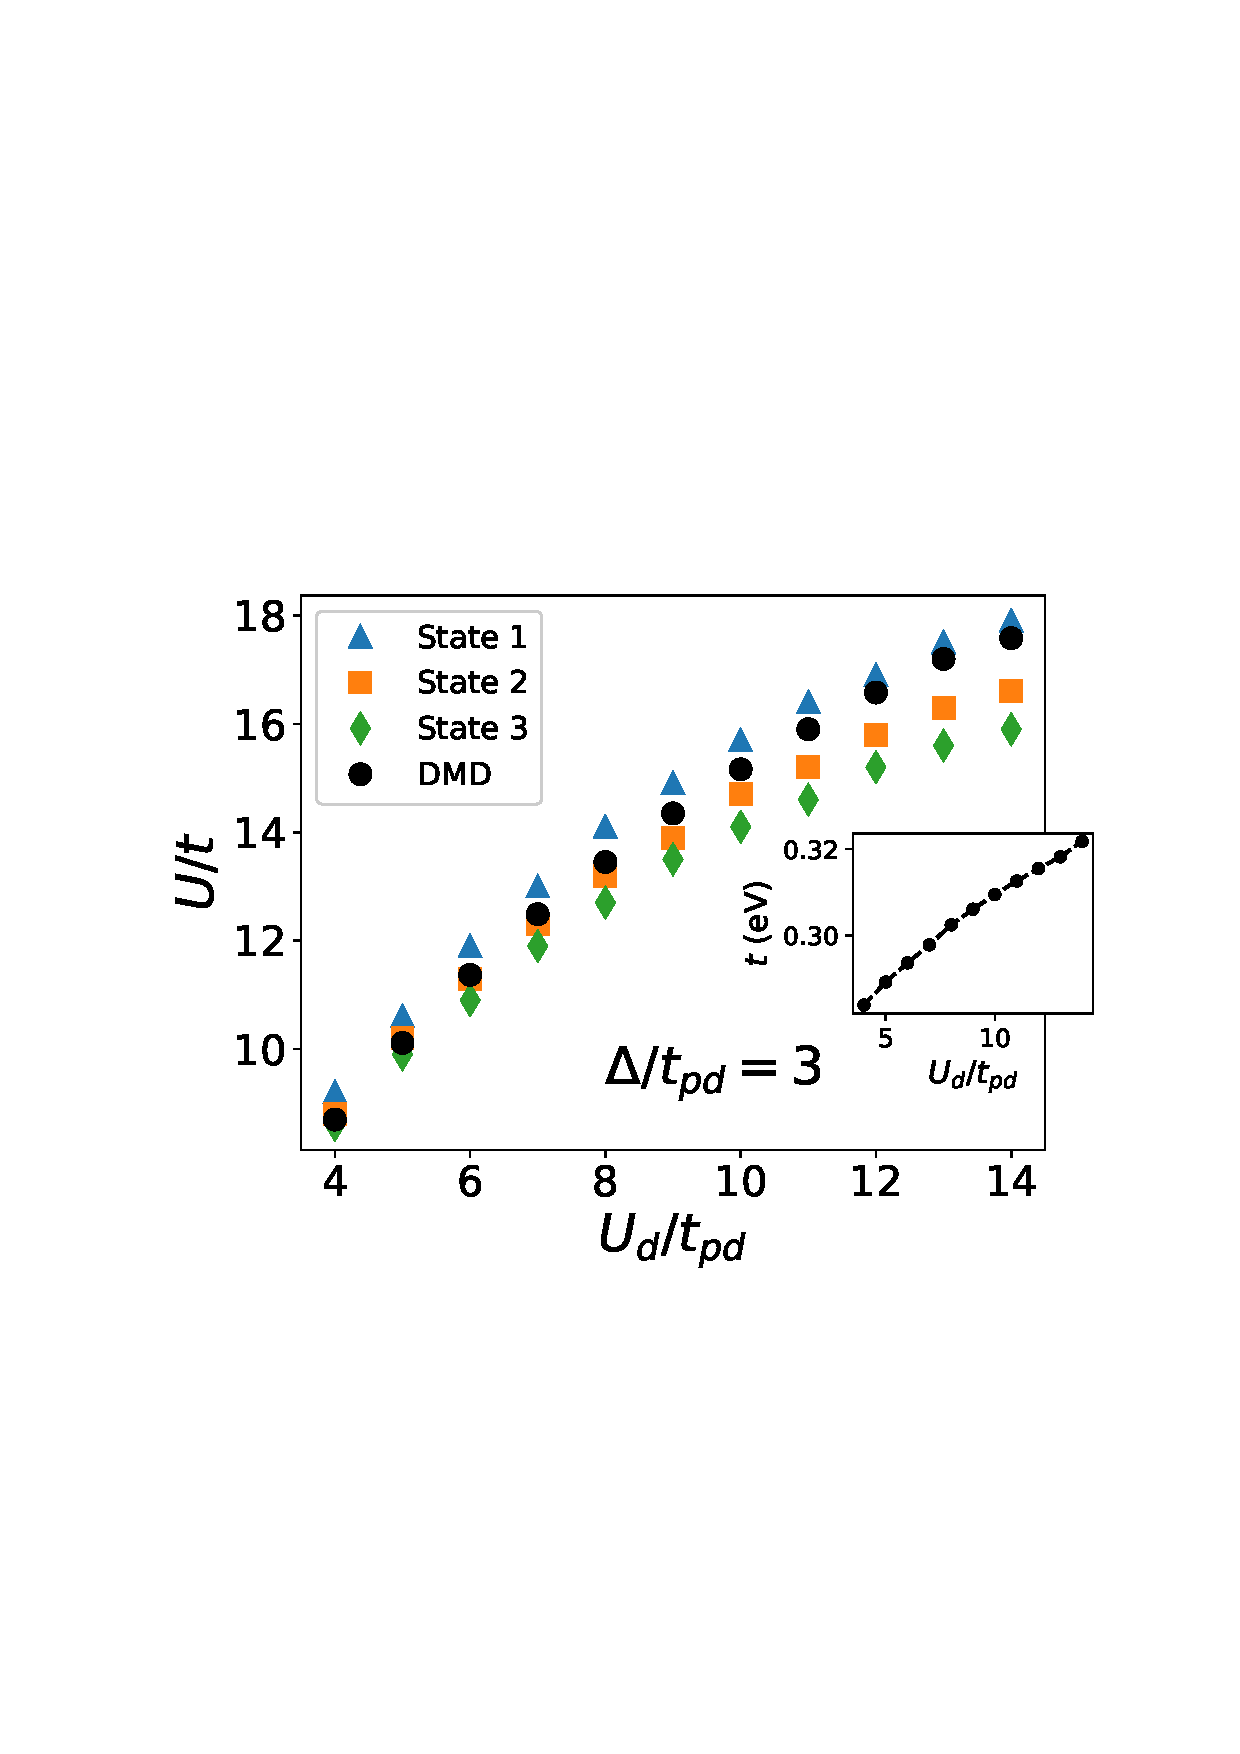
\includegraphics[width=0.48\linewidth]{./Figures/U_and_hopping_combined_vs_Ud_ep_3.pdf}
\includegraphics[width=0.50\linewidth]{./Figures/U_and_hopping_combined_vs_Ud_ep_5.pdf}
%\includegraphics[width=0.49\linewidth]{./Figures/downfolded_U_ep_3.pdf}
%\includegraphics[width=0.49\linewidth]{./Figures/Hopping_vs_U_ep_3.pdf}
%\includegraphics[width=0.49\linewidth]{./Figures/downfolded_U_ep_5.pdf}
%\includegraphics[width=0.49\linewidth]{./Figures/Hopping_vs_U_ep_5.pdf}
\caption{Downfolded values of the effective 1-band Hubbard $U/t$ and $t$ (inset) 
vs $U_d/t_{pd}$ for two representative values of $\Delta/t_{pd}$}
\label{fig:hamfitUdvary} 
\end{figure}	
 
Fig.~\ref{fig:hamfitepdvary} shows our results for the optimal 
transformation parameters ($\alpha$'s), $t$ and $U/t$ as a function of $\Delta/t_{pd}$
keeping $U_d/t_{pd}=8$ fixed. $\alpha_1$, which is the primary parameter that mixes (hybridizes) 
the copper and oxygen orbitals, \textit{decreases} as $\Delta/t_{pd}$ is increased. 
This is physically reasonable since an increasing difference in the single particle energies of the copper and oxygen orbitals 
means that it is even more energetically unfavorable to occupy the oxygen orbitals. 
Correspondingly the effective hopping between $\tilde{d}$ in the 
1-band model reduces and the effective $U/t$ increases. 

Next, in Fig.~\ref{fig:hamfitUdvary} we consider analogous results keeping $\Delta/t_{pd}$ fixed to two representative values, 
and varying $U_d/t_{pd}$. In both cases, $U/t$ increases dramatically with $U_d/t_{pd}$, but $t$ 
increases marginally little (similar results are seen for the dominant 
hybridization parameter $\alpha_1$). Also, the different estimates of $U/t$ are closer to each other 
for the case of larger $\Delta$ indicating the increased effectiveness of the 1-band model 
in the limit of large $\Delta$. 

A primary quality check for the model is its ability to reproduce the low energy spectrum. 
Fig.~\ref{fig:energyfit} shows the comparison of the 1-band vs 3-band model energy gaps 
(here only comprising of $6$ states). In all cases, the fit is reasonably good; 
the best fits seen at larger $U_d$ and larger $\Delta$ consistent with our expectations 
from the previous plots. We re-emphasize that once the density matrices were transformed 
only one parameter ($t$) was fit to match five energy gaps between the two models; this indicates 
it is thus an indicator of the success of the downfolding (rather than a result of overfitting). 

\begin{figure}[]
\centering
\includegraphics[width=0.325\linewidth]{./Figures/Gap_1_band_3_band_ep_3_number_5.pdf}
\includegraphics[width=0.325\linewidth]{./Figures/Gap_1_band_3_band_ep_3_number_9.pdf}
\includegraphics[width=0.325\linewidth]{./Figures/Gap_1_band_3_band_ep_3_number_2.pdf}
\includegraphics[width=0.325\linewidth]{./Figures/Gap_1_band_3_band_ep_5_number_5.pdf}
\includegraphics[width=0.325\linewidth]{./Figures/Gap_1_band_3_band_ep_5_number_9.pdf}
\includegraphics[width=0.325\linewidth]{./Figures/Gap_1_band_3_band_ep_5_number_2.pdf}
\caption{Comparison for energy gaps between the 3-band and 1-band Hubbard models 
using the optimized values of $U/t$ and $t$, for different $U_{d}/t_{pd}$ for $\Delta/t_{pd}=3$ (top row) 
and $\Delta/t_{pd}=5$ (bottom row)}
\label{fig:energyfit} 
\end{figure}	

\HJC {Predictivity} Ultimately, the whole reason for downfolding is to reduce the effective Hilbert space. 
Finally, we show that the obtained parameters are ....



\subsection{One dimensional hydrogen chain (Non-Eigenstate Fitting)}
%\subsection{One dimensional hydrogen chain (E-AIDMD)}
Let us consider the following single band model Hamiltonian,
\begin{eqnarray}\label{eq:h4model}
H &=& \sum_{i}\left\{-t[c^{\dagger}_{i\sigma}c_{i+1\sigma} +h.c.]+ Vn_{i}n_{i+1} + Un_{i\uparrow}n_{i\downarrow}+ J\vec \sigma_{i}\cdot \vec \sigma_{i+1}\right\} + C\,.
\end{eqnarray}
Here, $c_{i}$'s are Wannier orbitals generated from Kohn-Sham orbitals. We consider the case where the inter-atomic distance is relatively large, such that the system could be well described by a single band.  We start from the 4-site hydrogen chain with bond length equals to 2\AA with periodic boundary condition. We construct the Wannier orbitals by a unitary transformation of the four lowest energy Kohn-Sham states obtained from DFT/PBE calculation (2 occupied and 2 unoccupied). Fig.~\ref{fig:h4orb} shows the selected Kohn-Sham orbitals and constructed Wannier orbitals. 
\begin{figure}[hbt]
\centering
\subfigure[KS 1]{\includegraphics[width=0.20\linewidth]{h4_ks1.png}}\quad
\subfigure[KS 2]{\includegraphics[width=0.20\linewidth]{h4_ks2.png}}\quad
\subfigure[KS 3]{\includegraphics[width=0.20\linewidth]{h4_ks3.png}}\quad
\subfigure[KS 4]{\includegraphics[width=0.20\linewidth]{h4_ks4.png}}
\\
\subfigure[Wannier 1]{\includegraphics[width=0.20\linewidth]{h4_wan1.png}}\quad
\subfigure[Wannier 2]{\includegraphics[width=0.20\linewidth]{h4_wan2.png}}\quad
\subfigure[Wannier 3]{\includegraphics[width=0.20\linewidth]{h4_wan3.png}}\quad
\subfigure[Wannier 4]{\includegraphics[width=0.20\linewidth]{h4_wan4.png}}
\caption{Kohn-Sham orbitals (upper panel) from DFT calculations with PBE exchange-exchange correlation functional, and Wannier orbitals (lower panel) constructed through a unitary transformation of Kohn-Sham orbitals.}\label{fig:h4orb}
\end{figure}

%We will use the mentioned E-AIDMD method to downfold the ab initio system into the model Hamiltonian in Eq.~\eqref{eq:h4model} by matching the single-body energy spectra and the 1-body and 2-body reduced density matrices. The model Hamiltonian is solved by exact diagonization, whereas the \textit{ab initio} system is solved using diffusion Monte Carlo method with single Slater-Jastrow trial wave functions. 
%
%In our calculations, we used energies and RDMs of the following three states:
%\begin{subequations}
%\begin{eqnarray}
%S=0: \quad E = -2047.8(6) \text{mHa}; \\
%S=1: \quad E = -2038.9(5) \text{mHa}; \\
%S=2: \quad E = -1957.8(3) \text{mHa}.
%\end{eqnarray}
%\end{subequations}
%where S is the total angular moment of such the four-site hydrogen chain. In order to understand the relative importance of various two-body terms: (a) the on-site Hubbard interaction -- $\hat U$; (b) nearest neighbor Coulomb interaction -- $\hat V$; (c) nearest neighbor exchange -- $\hat J$, we compare the parameters obtained when downfolding the system to the following three different models with different two-body interactions,
%\begin{itemize}
%\item [(a)] \textbf{UVJ} model: onsite Hubbard interaction(U), nearest neighbor Coulomb (V) and exchange (J);
%\item [(b)] \textbf{UV} model: onsite Hubbard interaction(U), nearest neighbor Coulomb (V);  J is set to zero. 
%\item [(c)] \textbf{U} model: onsite Hubbard interaction(U). V and J are set to zero. 
%\end{itemize}
%
%The quality of downfolding is measured by the relative error of the two-body reduced density matrices, and the error of the eigen energies of the three states.
%\begin{eqnarray}
%R_{err} =\sqrt{\frac{\sum_{i,j,k,l}(M_{ijkl}^\text{ab initio} - M_{ijkl}^\text{model})^{2}}{\sum_{i,j,k,l}(M^\text{ab initio}_{ijkl})^{2} }}, \quad
%\Delta E = \sqrt{\sum_{i}|E_{i}^\text{ab initio} - E_{i}^{\text{model}}|^{2}}\,.
%\end{eqnarray}
%The resulting effective parameters are showed in Table.~\ref{tab:effm_hchain}. We see that all the three models can match the \textit{ab initio} data accurately. U model has relatively larger error in energy, but it is still comparable to the stochastic error from QMC (0.3 $\sim$ 0.5 mHa).
%
%\begin{table}[hbt]
%\centering
%\begin{tabular}{||l|c|c|c|c||c|c||}
%\hline
%Model & t & U & V & J & err(RDM) & err(energy)\\
%\hline
%\hline
%UVJ & 23.68 & 34.58 & 0.03 & -3.11 & 0.25\% & $10^{-13}$\\
%UV & 32.76 & 130.63 & 65.31 & / & 0.75\% & $10^{-13}$\\
%U & 37.45 & 114.62 & / & / & 0.26\% & $1.8$\\
%\hline
%\end{tabular}
%\caption{Parameters of effective Hamiltonian [mHa], and error of RDMs and energies [mHa].}\label{tab:effm_hchain}
%\end{table}
%
%%\subsection{Transferability of the model parameters to larger systems} 
%\begin{figure}[hbt]
%\centering
%\subfigure[]{\includegraphics[width=0.40\linewidth]{h4_transfer_rdm.png}}
%\subfigure[]{\includegraphics[width=0.40\linewidth]{h4_transfer_energy.png}}
%\caption{Errors of RDMs and energy for hydrogen chains with different number of sites: (a) relative error of two-body reduced density matrix; (b) error of eigen energy for $S=0$ and $S=1$ states per atom. the parameters used in model calculations are from 4-site chain.}\label{fig:h4transfer}
%\end{figure}
%In order to verify the transferability of the parameters for larger systems. We study longer chains (6-site, 8-site and 10-site) with the same inter-atomic distance (2\AA), and examine whether our parameters obtained from the 4-sites hydrogen chain is able to match the low energy physics of longer chains. We therefore, solve the model Hamiltonian with the parameters
%from Table.~\ref{tab:effm_hchain}, and examine the errors of the RDMs of S=0 and S=1 states. The results are
%shown in Fig.~\ref{fig:h4transfer}. As we can see, the error of the RDMs is around 10\%, indicating that the downfolding parameters from a smaller system is transferable to larger systems.
%Therefore, at $d=2$\AA, the hydrogen chain can be described by the extended Hubbard model \eqref{eq:h4model} very well. 

As an alternative to the model-fitting approach for hydrogen given above, we consider fitting a model to a periodic chain of 10 hydrogen atoms, but instead using low-energy states that do not explicitly target eigenstates of the Hamiltonian. In this example, we obtain single-particle Kohn-Sham orbitals from a set of spin-unrestricted and spin-restricted DFT-PBE calculations. With this set of orbitals, we produce a set of wave function states consisting of singles- and doubles- excitations to the Slater determinant. Allow $| S \rangle $ to be the Slater determinant formed from the Kohn-Sham orbitals, and orbitals $i$ and $j$ ($k$ and $l$) to be Kohn-Sham orbitals that are unoccupied (occupied) in the Slater determinant. We then produce new wave function states as singles excitations $|s \rangle$ and doubles excitations $| d \rangle$ excitations to the Slater determinant:
\begin{subequations}
\begin{eqnarray}
| s \rangle = & c^\dagger_{i \sigma} c_{k \sigma}   | S \rangle \\
| d \rangle = & \: c^\dagger_{i \sigma} c^\dagger_{j \sigma'} c_{k \sigma'} c_{l \sigma}   | S \rangle ,
\end{eqnarray}
\end{subequations}
where $\sigma$ and $\sigma'$ are spin indices and $c^\dagger$ ($c$) is a single-electron creation (destruction) operator. This technique does not access the explicit eigenstates of the Hamiltonian, but allows many more states to be sampled in the process of characterizing the low-energy Hilbert of space of the system. The localized orbital basis upon which the descriptors are calculated is obtained by generating intrinsic atomic orbitals (IAO) from the Kohn-Sham orbitals, and localizing them using the L\"owdin localization procedure.

Having produced a set of wave functions, we compute the total energies and descriptor values associated to each parameter that might appear in the model. The \textit{ab-initio} Hamiltonian is solved using diffusion Monte Carlo (DMC) with Slater-Jastrow trial wave functions. Fig.~\ref{fig:Histogram-of-Parameter-Values} shows distributions for the $U$ and $t$ descriptors computed using this set of singly- and doubly-excited wave function states.  Because these descriptors vary in value between the distinct states we have constructed, it is appropriate to include both within a single model.

There will exist some correlation between any two given descriptors. If two descriptors strongly covary with one another, then including both of them in a single model will introduce strong co-linearities, and produce aphysical parameter estimates. To control for this, we compute the covariance between descriptors prior to fitting a model, to verify that the descriptors are describing independent features of the wave function set. Fig.~\ref{fig:Cov-of-Descriptors} shows the absolute covariance of the hopping-$t$ descriptor with the $U$, $J$, and $V$ descriptors as a function of the separation distance between the hydrogen ions. We see that the covariance between the $t$ and $U$ descriptors is consistently low across all separation distances, indicating that these parameters are describing different wave function features. Therefore these descriptors are not strongly correlated with one another, and it is appropriate to include both in a single model.

Having computed the energies and descriptors for this set of wave functions, and verified the independence of the $U$ and $t$ descriptors, we fit a Hubbard-type model to describe the \textit{ab-initio} energetic results. Fig.~\ref{fig:RMS-Error-vs-Bond} shows the RMS error in the resultant $U$-$t$ model, relative to the \textit{ab-initio} DMC energetics, as a function of the hydrogen inter-atomic separation. We observe the the error is consistently less than 2 eV. The fitted value of the one-body hopping $t$ as a function of separation is shown in Fig.~\ref{fig:Parameters-vs-Bond-t}. As expected, the value of $t$ declines toward zero at larger separations. Hence, we see that the hydrogen chain can be well-described by a Hubbard-type model for a range of inter-atomic separations.

\begin{figure}
\centering
\includegraphics[scale=0.7]{Spin0_pbe_H_relation.pdf}
\caption{Histograms giving descriptor distributions for the one-body hopping $t$ and two-body Hubbard $U$ repulsion parameter for the periodic H$_{10}$ chain, with a lattice constant of $1.75$\AA.}\label{fig:Histogram-of-Parameter-Values}
 \end{figure}
 
 \begin{figure}
\centering
\includegraphics[scale=0.6]{t_covariance_vs_separation.pdf}
\caption{Covariance of the one-body hopping $t$ descriptor with the two-body $U$, $J$, and $V$ descriptors respectively, as a function of lattice constant for the periodic H$_{10}$ chain.  The covariance between the $t$ and $U$ is consistently small across all bond lengths.}\label{fig:Cov-of-Descriptors}
 \end{figure}
 
 \begin{figure}
\centering
\includegraphics[scale=0.6]{rms_ut_error_vs_separation_h_chain.pdf}
\caption{The RMS error in the fitted $U$-$t$ model for the periodic H$_{10}$ chain, relative to the \textit{ab-initio} energies. The RMS error is less than 1 eV for sufficiently long bond lengths.}\label{fig:RMS-Error-vs-Bond}
 \end{figure}
 
 \begin{figure}
\centering
\includegraphics[scale=0.6]{$t$_vs_separation_h_chain_ols.pdf}
\caption{The one-body hopping $t$ parameter as a function of lattice constant for the periodic H$_{10}$ chain, obtained from a fitted $U$-$t$ model. The parameter value declines to zero as the lattice constant increases.}\label{fig:Parameters-vs-Bond-t}
 \end{figure}

\subsection{Graphene and hydrogen honeycomb lattice}
\label{subsection:graphene}
Our third example highlights the role of the high energy 
degrees of freedom not present in the low energy description 
but which are instrumental in renormalizing the effective interactions. 
We demonstrate this by considering the case of graphene, and by 
comparing it to artificially constructed counterparts without the high energy electrons. 
Although many electronic properties of graphene can be adequately 
described by a noninteracting tight-binding model of $\pi$ electrons~\cite{Castro2009}, 
electron-electron interactions are crucial for explaining 
a wide range of phenomena observed in experiments~\cite{Kotov2012}. 
In particular, electron screening from $\sigma$ bonding renormalizes 
the low energy plasmon frequency of the $\pi$ electrons~\cite{Zheng2016}. 
In fact a system of $\pi$ electrons with bare Coulomb interactions has been shown to be an insulator instead of a semimetal~\cite{DrutPRL2009, DrutPRB2009,  Smith2014, Zheng2016}. 
Using DMD, we demonstrate how the screening effect of $\sigma$ electrons is manifested in the low energy effective model of graphene. 

In order to disentangle the screening effect of $\sigma$ electrons from the bare interactions 
between $\pi$ electrons, we apply DMD to three different systems, graphene, $\pi$-only graphene, and a honeycomb lattice of hydrogen atoms.  
In $\pi$-only graphene, the 
$\sigma$ electrons are replaced with a static constant negative charge background. 
The role of $\sigma$ electrons is then clarified by comparing the effective model Hamiltonians of these two systems. 
The hydrogen system we study has the same lattice constant $a=2.46$~\AA~as graphene, 
which has a similar Dirac cone dispersion as graphene~\cite{Zheng2016}. 

By constructing the one-body space by Wannier localizing Kohn-Sham orbitals obtained from DFT calculations (see Figure~\ref{fig:honeycomb_wan}), 
we verify that the low energy degrees of freedom correspond to the $\pi$ orbitals in graphene and 
its $\pi$-only system and $s$ orbitals in hydrogen; these enter the effective one-band Hubbard model description in Eq.~\eqref{eq:oneband}. 
Due to the vanishing density of states at the Fermi level, the Coulomb interaction remains long-ranged, 
in contrast to usual metals where the formation of electron-hole pairs screens the interactions strongly~\cite{Zheng2016}. 
However, for certain aspects, the long ranged part can be considered as renormalizing the 
onsite Coulomb interaction $U$ at low energy~\cite{Schuler2013, Changlani2015}. 

\renewcommand{\subfigimg}[3][,]{%
  \setbox1=\hbox{\includegraphics[#1]{#3}}% Store image in box
  \leavevmode\rlap{\usebox1}% Print image
  \rlap{\hspace*{20pt}\vspace*{18pt}\raisebox{\dimexpr\ht1-1.37\baselineskip}{#2}}% Print label
  \phantom{\usebox1}
}
\begin{figure}[hbt]
\centering
 \begin{tabular}{@{}p{0.90\linewidth}@{\quad}p{\linewidth}@{}}
   \subfigimg[clip, width=0.45\textwidth]{(A)}{./Figures/c_pi.eps}
   \subfigimg[clip, width=0.45\textwidth]{(B)}{./Figures/h_wan.eps}
 \end{tabular}
\caption{Wannier orbitals constructed from Kohn-Sham orbitals: (A) graphene $\pi$ orbital; (B) hydrogen $s$ orbital. }
\label{fig:honeycomb_wan}
\end{figure}

To estimate the one-band Hubbard parameters, we used the DMD method using a set of 50 Slater-Jastrow wave functions that correspond 
to the electron-hole excitations within the $\pi$ channel for the graphene systems 
or $s$ channel for the hydrogen system. In particular, for graphene, 
the Slater-Jastrow wave functions are constructed from occupied $\sigma$ bands and occupied $\pi$ bands, whereas for $\pi$-only 
graphene, Slater-Jastrow wave functions are constructed from occupied $\pi$ Kohn-Sham orbitals of graphene. The \textit{ab initio} simulations 
were performed on a $3\times3$ cell (32 carbons or hydrogens) and the energy and RDMs of these wave functions were
evaluated with VMC. The error bars on our downfolded parameters are estimated using the jackknife method \cite{Jackknife1981}.
The results from our calculations are summarized in Figure~\ref{fig:ne_aidmd_gh}.

\renewcommand{\subfigimg}[3][,]{%
  \setbox1=\hbox{\includegraphics[#1]{#3}}% Store image in box
  \leavevmode\rlap{\usebox1}% Print image
  \rlap{\hspace*{42pt}\vspace*{12pt}\raisebox{\dimexpr\ht1-1.37\baselineskip}{#2}}% Print label
  \phantom{\usebox1}
}
\begin{figure}[hbt]
\centering
  \begin{tabular}{@{}p{0.95\linewidth}@{\quad}p{\linewidth}@{}}
    \subfigimg[clip, width=0.325\linewidth]{(A)}{./Figures/grp_all_tu.eps}
    \subfigimg[clip, width=0.325\linewidth]{(B)}{./Figures/grp_pi_tu.eps}
    \subfigimg[clip, width=0.325\linewidth]{(C)}{./Figures/h_tu.eps}
    \end{tabular}
\caption{Comparison of \textit{ab initio} ($E[\psi]$) and fitted energies ($E_{eff}[\psi]$) 
of the 3$\times$3 periodic unit cell of graphene and hydrogen lattice: (A) graphene; (B) $\pi$-only graphene; (C) hydrogen lattice.}\label{fig:ne_aidmd_gh}
\end{figure}

We find that the one-band Hubbard model describes graphene and hydrogen very well, as is seen from the fact that $R^2$ is close to 1 for the fits. 
Our fits are shown in Figure~\ref{fig:ne_aidmd_gh}. For both graphene and hydrogen, $U/t$ is smaller than the critical value of the 
semimetal-insulator transition $(U/t)_c \approx 3.8$ for the honeycomb lattice~\cite{Sorella2012}, 
which is consistent with both systems being semimetals. The Fermi velocity of graphene estimated from the dowfolded parameters [$t=3.62(1)$ eV and $U=7.21(4)$ eV] using the 
Hartree-Fock approximation is $1.2\times 10^{6}$ m/s, which is consistent with the experimental value $1.1 \times 10^6$ m/s~\cite{Siegel2011}. 
Graphene and hydrogen have similar hopping constant $t$, consistent with the fact that they have similar band dispersions near the Dirac point. 
However, the difference in their high energy structure manifests itself as differently renormalized electron-electrons interactions, 
explaining the difference in $U$. Most prominently, the $\pi$-only system has much larger $U/t$ ($\sim4.9$) compared to graphene, 
which is large enough to push it into the insulating (antiferromagnetic) phase.
Thus, downfolding shows the clear significance of $\sigma$ electrons in renormalizing the effective onsite interactions of the $\pi$ orbitals, making graphene a weakly interacting semimetal instead of an insulator.  



\section{Conclusion and Future prospects}
To summarize, we have explained the AIDMD method that we have been developing, primarily in conjunction with the 
\emph{ab-initio} QMC approach. The practical motivation is to take data from first principles (continuum) 
calculations as inputs for lattice model (discrete) methods. 
Since one is mapping a many body problem to a few body one, the relevant quantities of interest are 
the reduced density matrices associated with the many-body wavefunctions projected to a one-body space. 
The density matrix based approach is appealing as it is democratic 
in the determination of the hopping and interaction parts of the effective Hamiltonian, and provides multiple 
checks on its validity. We have discussed three representative examples to discuss the conceptual and algorithmic aspects of AIDMD. 

What sort of accuracy should one expect with effective Hamiltonians and AIDMD? The holy grail of quantum chemistry 
and electronic structure is to obtain an energy of 1 mHa (0.027 eV) per atom; this 
remains an open challenge despite decades of work. The effective Hamiltonian approach largely ameliorates this problem,  only 
relative energies are important, neither the total energy (nor its accuracy) is of particularly 
fundamental interest. This, of course, is contingent on the cancellation of the large energy associated with the core electrons, 
whose role is to primarily renormalize the interactions between the active (valence) electrons. This aspect can also 
be a major limitation when the core and active electrons are strongly entangled i.e when the separation of energy 
scales is not prominent (in which case an energy-dependent description may be needed). 
Thus, it is possibly best suited for extended systems (solids) where this separation exists. 
In our view, AIDMD (and downfolding in general) opens up many avenues for determination of physical 
quantities not easily calculated in ground state approaches. Our experience suggests excitation spectra 
can be accurately determined to 0.2 eV (or less)~\cite{Changlani2015} and potentially improved with 
more \emph{ab-initio} data and more refined effective Hamiltonians.  
%It is also possibly best suited for extended systems (solids) where there is often a clear separation of energy scales associated with the 
%core, active (valence) and virtual electronic spaces. 

Finally we would like to emphasize that AIDMD, though conceptually simple, 
is still a method in its development stages, with room for algorithmic improvements and new applications. It suffers 
from the usual problems of optimization and overfitting, but with advances in these fields we believe some of these major 
concerns may become less problematic. Some of the issues that need further research are,
\begin{itemize} 
	\item Construction of wavefunction database:
	The AIDMD method relies crucially on the availability of a low energy space of \emph{ab initio} wavefunctions, 
	which despite not being eigenstates, reveal the nature of the effective Hamiltonian. Automating its construction 
	remains somewhat challenging. We propose Slater Jastrow wavefunctions and deforming the orbitals entering the Slater 
	determinant as one way of probing the low energy manifold.
	\item Optimal choice of active orbitals (one body space):
	In the present work, we chose DFT orbitals (in a certain energy window) and localized them to get the one body orbitals. 
	The choice could only be justified based on looking at the trace of the 1-RDM and ensuring that it 
	equalled the expected number of electrons. We expect to use intrinisic atomic orbitals (pointed out to us by G. K. Chan) which 
	mitigate this issue. 
	\item Form of the low energy model Hamiltonian:
	Extensive work in the literature has been devoted to parameterizing compact effective Hamiltonians~\cite{Georges, Oles, Coury}. 
	Since the low energy effective Hamiltonian is not unique, there is not necessarily one right way of downfolding. 
	One could catalogue all functional forms based on previous parameterizations 
	or there may be some merit in determining the minimal description with fewest non zero parameters.
	Note that most models for strong correlation \emph{assume} two body forms. While this appears to work well in practice, 
	it is by not guaranteed on mathematical grounds. (Even though the Coulomb operator is two body, 
	its low energy description need not be.)
	\item Other (non QMC) wavefunction based electronic structure methods:
	There are several wavefunction based quantum chemistry 
	methods for electronic structure like coupled cluster and ab-initio DMRG which work primarily 
	directly in orbital space. These could also be potentially explored in conjunction with AIDMD.
	
\end{itemize} 

In terms of applications, we hope the method will be eventually applied to solids involving transition 
metals and/or rare earth elements, which are in the strongly correlated regime due to the presence of localized orbitals. 
Some challenging areas include,
\begin{itemize} 
	\item Spin models for magnetism: 
	The magnetism associated with strongly correlated Mott insulators, compounded by effects such as geometrical frustration, 
	is highly non trivial and has become an active area of research in its own right. 
	%This is compounded by 
	%the presence of geometric frustration, impurities and defects and 
	%spin-orbital effects. 
	For example, the two dimensional kagome lattice planes in 
	herbertsmithite harbor an exotic topological phase of matter - a "quantum spin liquid". While our understanding is primarily 
	from Heisenberg models~\cite{Yan_Huse_White, Changlani_kagome}, 
	contentious issues plague a complete understanding and connection to experiment (there has been recent progress 
	in downfolding herbertsmithite~\cite{Jeschke}). 
	Other areas of application include pyrochlore iridates and titanates and Kitaev materials. 
	We caution that relevant energy scales associated with magnetism can be $0.1$ meV or less, and no electronic structure 
	method is currently that accurate. It may thus be necessary to perform multiple downfolding steps to map from 
	the Schrodinger equation to a spin model.
	\item Multiband models for superconductors:
	As previously mentioned, unconventional (non BCS) superconductivity in materials such as the cuprates and iron based 
	pntictides has fuelled the study of strongly correlated systems.
	Several parameter sets exist in the literature for multi-band models, but it appears that there is little universal consensus. 
	We are optimistic that additional \emph{ab-initio} inputs from AIDMD will help constrain the part of parameter 
	space relevant for these materials. Trends of the parameters (and the effectiveness of the three band 
	or one band model itself) with pressure dependence and doping remain largely unexplored.  
	%\item Quantum computing (\HJC{tell me if this one is too weird}) : 
	%Quantum computers have been heralded as the future of computing with many promising advances. 
	%There has been progress in the simulation of small molecules in compact basis sets, but scalability (needed for solids) 
	%remains an issue. Downfolding macould help in the reduction in the number of active orbitals 
\end{itemize} 


\bibliographystyle{unsrt}
\bibliography{refs}

\end{document}
